\chapter{随机变量的数字特征}
\section{数学期望}
\subsection{随机变量的数学期望}
\dfn{}{
    设离散型随机变量$X$的概率分布为
    \[\Pr{X = x_i} = p_i, \, i=1, 2, \ldots\]
    若级数$\displaystyle\sum_{i=1}^{\infty}x_ip_i$\emph{绝对收敛}, 则定义$X$的\vocab{数学期望}为
    \begin{equation}
        \EE{X} = \sum_{i}x_ip_i.
    \end{equation}
}
\leftnote[-2.8cm]{复习:绝对收敛:\\$\sum_{i=1}^{+\infty}\abs{x_ip_i}<\infty$}
\leftnote[-1.6cm]{$\EE{X}, \mathrm{E}(X), EX$都是等价的写法.}

上述定义限于离散型随机变量.考虑连续型随机变量$X$, 其PDF为$f(x)$. 在数轴上取一段长度为$\Delta x\to 0$的区间$[x, x+\Delta x]$, 则$X$落入该区间的概率为
\[\Pr{x\leq X\leq x+\Delta x} = \int_{x}^{x+\Delta x}f(x)\dd{x}\approx f(x)\Delta x.\]
\leftnote{这称为离散化}
在数轴上取无限多段这样的小区间并对概率求和, 我们有
\[\sum_ix_if(x_i)\Delta x_i \approx \int_{\RR}xf(x)\dd{x}.\]
因此可以得到定义:
\leftnote{并非所有随机变量都有数学期望}
\dfn{}{
    设$X$是连续型随机变量, PDF为$f(x)$, 若上述积分\emph{绝对收敛}, 定义$X$的\vocab{数学期望}为
    \begin{equation}
        \EE{X} = \int_{\RR}xf(x)\dd{x}.
    \end{equation}
}
\subsection{随机变量函数的数学期望}
对于随机变量$X$的函数$Y = g(X)$, 我们可以通过定义求出$X$的分布而求出$Y$的分布, 进而由定义得$Y$的数学期望$\EE{g(X)}$, 这做法较繁.\newpage
\thm{}{
    设$X$是一个随机变量, $Y=g(X)$, 且$E(Y)$存在, 于是\\
    (1)若$X$为离散型随机变量:
    \begin{equation}
        \EE{Y}= \EE{g(X)} = \sum_{i}g(x_i)p_i,
    \end{equation}
    (2)若$X$为连续型随机变量:
    \begin{equation}
        \EE{Y} = \EE{g(X)} =\int_{\RR}g(x)f(x)\dd{x}.
    \end{equation}
}
推广至二维: 设$(X, Y)$是二维随机变量, $Z=g(X, Y)$, 若$\EE{Z}$存在, 则\\
(1)若为离散型:
\begin{equation}
    \EE{Z} = \EE{g(X, Y)} = \sum_{i}\sum_{j}g(x_i, y_j)p_{ij},
    \label{eq:4.5}
\end{equation}
(2)若为连续型:
\begin{equation}
    \EE{Z} = \EE{g(X, Y)} = \iint_{\RR[2]}g(x, y)f(x, y)\dd{\sigma}.
\end{equation}
\textbf{注意}\quad 实际做题中, 积分区域$D\subseteq \RR$, 根据\emph{\color{red}所要求期望的随机变量来决定积分次序}.\;\Eg\, $\EE{X}$---先对$y$积分, 再对$x$积分;\, $\EE{Y}$---先对$x$积分, 再对$y$积分;\, $\EE{XY}$---两者谁先皆可, 但注意不满足Fubini定理的函数.
\subsection{数学期望的性质}
\begin{enumerate}
    \item $\EE{c} = c$ (c为常数, 下同);
    \item $\EE{cX} = c\EE{X}$;
    \item $\EE{X+Y} = \EE{X} + \EE{Y}$;
    \item 若$X, Y$相互独立, 则$\EE{XY} = \EE{X}\EE{Y}$.
\end{enumerate}
\exc{P\textsubscript{85}5}{
    设随机变量$X$的分布律为
    \begin{center}
        \begin{tabular}{@{}llll@{}}
            \toprule
            $X$   & $-2$  & $0$   & $2$   \\ \midrule
            $p_i$ & $0.4$ & $0.3$ & $0.3$ \\ \bottomrule
        \end{tabular}
    \end{center}
    求$\EE{X}, \EE{X^2}, \EE{3X^2+5}$
}
\sol{
    由题意得, $\EE{X} = -0.2$.
    \;\;设$Y=X^2$, 由\eqref{eq:4.5}得$\EE{X^2} = 2.8$.
    \;\;由性质123得$\EE{3X^2+5} = 3\EE{X^2} + \EE{5} = 13.4$.
}
\exc{P\textsubscript{85}10}{
    设$(X, Y)$的概率密度为
    \begin{equation*}
        f(x, y) = \begin{cases}
            12y^2, & 0\leq y\leq x\leq 1, \\
            0,     & \mbox{otherwise}
        \end{cases}
    \end{equation*}
    求$\EE{X}, \EE{Y}, \EE{XY}, \EE{X^2 + Y^2}$.
}
\sol{由题意得, 实际的积分区域为$x$轴, $x=1$和$y=x$围成的三角形区域$D$.\\
    (1)求$\EE{X}$, 由定义可得$\EE{X} = \int_{-\infty}^{+\infty}xf_X(x)\dd{x}$, 展开有
    \[\EE{X} = \iint_{\RR[2]}xf(x, y)\dd{x}\dd{y}\]
    \leftnote{$D_1 = D_2$, 分开写是强调\emph{积分次序}.}
    注意到$f(x, y)$在$D_1 = \{0\leq x\leq 1, 0\leq y\leq x\}$上不为$0$, 计算得$\EE{X} = \dfrac{4}{5}$.\\
    (2)同理, 求$\EE{Y}$, $D_2 = \{0\leq y\leq 1, y\leq x\leq 1\}$.可得
    \[\EE{Y} = \underbrace{\int_{0}^{1}\int_{y}^{1}}_{D_2}yf(x, y)\dd{x}\dd{y} = \frac{3}{5}.\]
    (3)由于$f_X(x)f_Y(y)\neq f(x, y)$, $X, Y$不具有独立性, 无法使用性质4.\\
    \leftnote{这个次序计算简单}
    由于积分次序不影响结果, 因此先积$y$再积$x$可得
    \[\EE{XY} = \iint_{D_1}xyf(x, y)\dd{\sigma} = \frac{1}{2}.\]
    (4)由性质3得$\EE{X^2 + Y^2} = \EE{X^2} + \EE{Y^2}$.由 (1) (2)可得
    \[\EE{X^2 + Y^2} = \iint_{D_1}x^2f(x, y)\dd{\sigma}+\iint_{D_2}y^2f(x, y)\dd{\sigma} = \frac{16}{15}.\]
}
\section{方差}
\subsection{方差的定义}
\dfn{方差}{
    设$X$是一个随机变量, 若$\EE[2]{X-\mu}$存在, 则称其为$X$的\vocab{方差}, 记为$\Var{X}$, 其中$\mu = \EE{X}$.
    方差亦记作$\operatorname{Var}X, D(X), DX$.\\
    方差的算数平方根$\sqrt{\Var{X}}$称为$X$的\emph{标准差}, 记为$\sigma_X$.
}
\leftnote{常见分布的期望和方差见书$P_{215}$}
方差刻画了随机变量$X$的取值与其期望$\mu$的偏离程度, 方差越大, 随机变量的取值越分散. 而且, 若$\Var{X} = 0$, 则随机变量$X$一定取常数值, 此时$X$不是随机变量.
\subsection{方差的计算}
若$X$是\emph{离散型}随机变量, 其分布律为$\Pr{X=x_i} = p_i, \, i=1, 2, \ldots$, 则
\begin{equation}
    \Var{X} = \EE[2]{X-\mu} = \sum_{i}(x_i-\mu)^2p_i.
\end{equation}

若$X$是\emph{连续型}随机变量, 其概率密度为$f(x)$, 则
\begin{equation}
    \Var{X} = \EE[2]{X-\mu} = \int_{\RR}(x-\mu)^2f(x)\dd{x}.
\end{equation}
由数学期望的性质可得方差计算的重要公式:
\begin{equation}
    \Var{X} = \EE{X^2} - \EE[2]{X}.
\end{equation}
\pf{证明}{
    \begin{align*}
        \Var{X} & = \EE[2]{X-\mu} = \EE{X^2 - 2\mu X + \mu^2} \\
                & = \EE{X^2} - 2\mu\EE{X} + \mu^2             \\
                & = \EE{X^2} - 2\mu^2 + \mu^2                 \\
                & = \EE{X^2} - \EE[2]{X}.
    \end{align*}
}
\qs{Poisson分布}{
    设$X\sim P(\lambda)$, 求$\EE{X}, \Var{X}$.
}
\sol{
    随机变量$X$的分布律为
    \begin{equation*}
        \Pr{X=k} = \frac{\lambda^k}{k!}e^{-\lambda}, \, k=0, 1, \ldots;\;\lambda > 0.
    \end{equation*}
    \begin{align*}
        \text{由定义得\;}
        \EE{X}   & = \sum_{k = 0}^{\infty}k\dfrac{\lambda^ke^{-\lambda}}{k!} = \lambda e^{-\lambda}\sum_{k = 1}^{\infty}\dfrac{\lambda^{k-1}}{(k-1)!} = \lambda e^{-\lambda}\cdot e^{\lambda} = \lambda,            \\
        \EE{X^2} & = \EE{X(X - 1) + X} = \EE{X(X - 1)} + \EE{X}                                                                                                                                                     \\
                 & = \sum_{k = 0}^{\infty}k(k - 1)\dfrac{\lambda^ke^{-\lambda}}{k!} + \lambda = \lambda^2e^{-\lambda}\underbrace{\sum_{k = 2}^{\infty}\dfrac{\lambda^{k-2}}{(k-2)!}}_{\text{Poisson分布}=1} + \lambda \\
                 & = \lambda^2e^{-\lambda}\cdot e^{\lambda} + \lambda = \lambda^2 + \lambda,                                                                                                                        \\
    \end{align*}
    \begin{equation}
        \text{故方差\;}\Var{X} = \EE{X^2} - \EE[2]{X} = \lambda.
    \end{equation}

}
\qs{均匀分布}{
    设$X\sim U(a, b)$, 求$\EE{X}, \Var{X}$.
}
\sol{
    $X$的概率密度为
    \begin{equation*}
        f(x) = \begin{cases}
            \dfrac{1}{b-a}, a<x<b, \\
            0, \text{otherwise}.
        \end{cases}
    \end{equation*}
    \begin{equation}
        \text{而\;}\Var{X} = \EE{X^2} - \EE[2]{X} = \int_{a}^{b}x^2\dfrac{1}{b-a}\dd{x} - \left(\dfrac{a+b}{2}\right)^2 = \dfrac{(b- a)^2}{12}.
    \end{equation}
}
\subsection{方差的性质}
\begin{enumerate}
    \item $\Var{c} = 0$;
    \item $\Var{X}\geq 0$;
    \item $\Var{cX} = c^2\Var{X}$;
    \item $\Var{c + X} = \Var{X}$;
    \item $\Var{X+Y} = \Var{X} + \Var{Y} + 2\operatorname{Cov}(X, Y)$;
    \item 若$X, Y$相互独立, 则$\Var{X+Y} = \Var{X} + \Var{Y}$.
\end{enumerate}
第六个性质可以推广到$n$维, 即若$X_1, X_2, \ldots, X_n$相互独立, 则
\begin{equation*}
    \Var{\sum_{i=1}^{n}X_i} = \sum_{i=1}^{n}\Var{X_i}.
\end{equation*}

\exc{P\textsubscript{90}8}{
    设$X\sim N(1, 2)$, $Y\sim E(3)$, 且$X, Y$相互独立, 求$\Var{XY}$.
}
\sol{
    (分析法)要求$\Var{XY}$, 即求$\EE{XY^2} - \EE[2]{XY}$. 因为$X, Y$独立, 则
    \begin{align*}
        \Var{XY}                                & = \EE{XY^2} - \EE[2]{X}\EE[2]{Y}.                                                        \\
        \intertext{因为$X, Y$独立, 则$X^2, Y^2$也独立.有}
        \leftnote{定理 (3.2.2)}
                                                & = \EE{X^2}\EE{Y^2} - \EE[2]{X}\EE[2]{Y}.                                                 \\
        \intertext{$X^2, Y^2$这俩玩意积不出来, 继续展开有}
                                                & = \left(\EE[2]{X} + \Var{X}\right)\left(\EE[2]{Y} + \Var{Y}\right) - \EE[2]{X}\EE[2]{Y}. \\
        \text{已知$\EE{X} = 1, \, \EE{Y} = 3$, 得} & = 27.
    \end{align*}
}

若设$f(x) = \EE[2]{X -x}, \, x\in \RR$, 求导可证明$f(x)$在$x = \mu$处取得最小值, 即$\Var{X}$在$\mu$处取得最小值, 这说明随机变量的取值\uwave{对其数学期望的偏离程度比对其他任何值的偏离程度都要小}.
\thm{}{
    若随机变量序列$\{X_n\}\sim N$, 且相互独立, 则其和常数的\emph{线性组合}仍然服从正态分布.
    \begin{equation}
        \ie\;\;\bmA\times\begin{pmatrix}
            X_1 \\ X_2 \\ \vdots \\ X_n
        \end{pmatrix}\sim N, \text{where\;} \bmA = \begin{pmatrix}
            a_1 & a_2 & \cdots & a_n
        \end{pmatrix}.
    \end{equation}
}
\ex{P\textsubscript{91}4}{
    若$X_i\sim N(\mu_i, \sigma_i^2), \, i=1, 2, \ldots, n$, 且相互独立, 求$Y=\sum_{i=1}^{n}(a_iX_i + b_i)$服从什么分布.
}
\sol{
    由题意, $Y$是$X$的一个线性组合, 所以$Y$服从正态分布.
    \leftnote{定理 (4.2.1)}
    \begin{align*}
        \EE{Y}  & = \sum_{i=1}^{n}a_i\EE{X_i} + \sum_{i=1}^{n}b_i, \\
        \Var{Y} & = \sum_{i=1}^{n}a_i^2\Var{X_i}.
    \end{align*}
    \[\tf\ \ Y\sim N\left(\sum_{i = 1}^{n}(a_i\mu_i + b_i), \sum_{i=1}^{n}a_i^2\sigma_i^2\right)\]
}
\section{大数定律与中心极限定理}
\subsection{Chebyshev不等式}
\thm{Chebyshev不等式}{
    设随机变量$X$的期望为$\mu$, 方差为$\sigma^2$, 则对任意$\epsilon > 0$, 有
    \begin{equation}
        \Pr{\abs{X-\mu}\geq \varepsilon}\leq \frac{\sigma^2}{\varepsilon^2}.
    \end{equation}
}
\newpage

\begin{wrapfigure}[4]{r}{.4\textwidth}
    \centering
    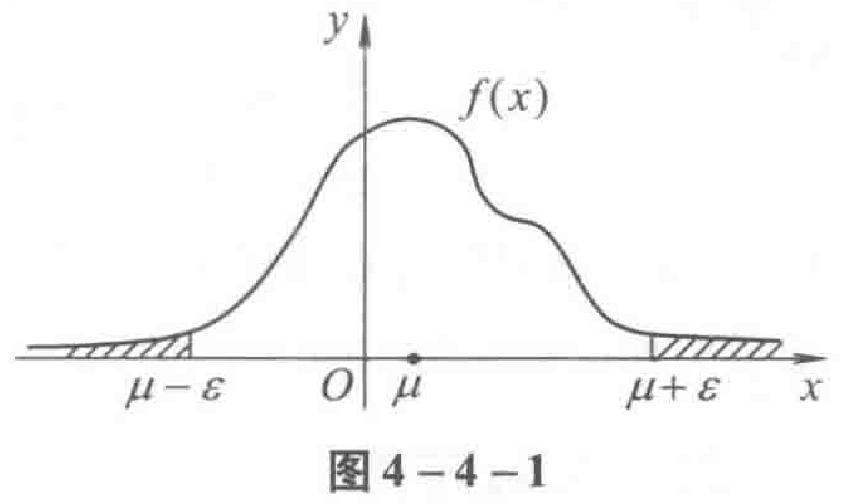
\includegraphics[scale=.4]{chebyshev}
    \centering
    \caption{$f(x)$示意}
\end{wrapfigure}
这个不等式从直观上表示事件$X$的取值都落在$\mu$的一个邻域$(\mu -\epsilon, \mu +\epsilon)$\emph{之外} (阴影部分)的概率. 它同时指出随机变量$X$的方差越小, 事件$\{\abs{X-\mu}<\epsilon\}$发生的概率越大, 即$X$的取值基本上集中在$\mu$的邻域内. 因此称方差刻画了随机变量的离散程度.

只证连续型的情况. 设$X$的概率密度为$f(x)$, 则
\pf{证明}{
    \begin{align*}
        \begin{split}
            \Pr{\abs{X-\mu}\geq \epsilon} & = \int_{\abs{x-\mu}\geq\epsilon}f(x)\dd{x}.
        \end{split}
        \intertext{放缩, 取$k = \dfrac{\abs{x-\mu}^2}{\epsilon^2}$. (因为$X$都落在邻域外, 则$k > 1$.)}
        \begin{split}
             & \leq\int_{\abs{x-\mu}\geq\epsilon}kf(x)\dd{x}
        \end{split}
        \begin{split}
             & \text{再次放缩, 变大区间}                                                                                            \\
             & \leq\dfrac{1}{\epsilon^2}\underbrace{\int_{\RR}(x-\mu)^2f(x)\dd{x}}_{\Var{X}} = \dfrac{\sigma^2}{\epsilon^2}
        \end{split}
    \end{align*}
}
\subsection{大数定律}
\mlemma{随机变量序列相互独立}{
    若对于任意$n>1$, $X_1, X_2, \ldots, X_n$都相互独立, 则称$X_1, X_2, \ldots, X_n, \ldots$是相互独立的.
}
\thm{大数定律}{
    设随机变量$X_1, X_2, \ldots, X_n, \ldots$相互独立, 且具有相同的期望和方差
    \[\EE{X_i} = \mu, \, \Var{X_i} = \sigma^2, \, i=1, 2, \ldots.\]
    记$\displaystyle Y_n = \dfrac{1}{n}\sum_{i=1}^{n}X_i$, 则对任意$\epsilon > 0$, 有
    \begin{equation}
        \lim_{n\to\infty}\Pr{\abs{Y_n - \mu} < \epsilon} = 1
    \end{equation}
}
\pf{证明}{
    由$Y_n$的式子可以知道
    \begin{align*}
        \EE{Y_n} = \dfrac{1}{n}\sum_{i = 1}^{n}\EE{X_i} = \mu, &  & \Var{Y_n} = \dfrac{1}{n^2}\sum_{i = 1}^{n}\Var{X_i} = \dfrac{\sigma^2}{n},
    \end{align*}
    由Chebyshev不等式可得
    \begin{align*}
        \Pr{\abs{Y_n - \mu} < \epsilon} & \geq 1 - \Pr{\abs{Y_n - \mu} \geq \epsilon}          \\
                                        & \geq 1 - \dfrac{\Var{Y_n}}{\epsilon^2}               \\
                                        & \geq 1 - \dfrac{\sigma^2}{n\epsilon^2}. \tag{$\ast$}
    \end{align*}
    夹逼法, $(\ast)$式两边取极限, 且因为概率不可能大于$1$,
    \begin{align*}
        1\geq & \lim_{n\to\infty}\Pr{\abs{Y_n - \mu} < \epsilon}\geq\lim_{n\to\infty}1 - \dfrac{\sigma^2}{n\epsilon^2} = 1. \\
        \tf   & \lim_{n\to\infty}\Pr{\abs{Y_n - \mu} < \epsilon} = 1.
    \end{align*}
}

这表明对任意$\epsilon > 0$, 事件$\abs{Y_n - \mu} < \epsilon$发生的概率很大 ($Y_n$的取值一定落在$\mu$的邻域内),
当$n$很大时, $Y_n$集中于$\mu$.
像这样表现的收敛性成为随机变量序列$Y_1, Y_2, \ldots, Y_n, \ldots$\vocab{依概率收敛}于$\mu$, 记为
\begin{equation}
    Y_n\xrightarrow{P}\mu.
\end{equation}
这还表明, 随机变量$X_1, X_2, \ldots, X_n$的算术平均值序列${Y_n}$依概率收敛于$\mu$.
\cor{Bernoulli定理}{
    设$n_A$是$n$重Bernoulli试验中事件$A$发生的次数, $p$是事件$A$在每次试验中发生的概率 ($n_A\sim b(n, p)$), 则对任意的$\epsilon > 0$, 有
    \begin{equation}
        \lim_{n\to\infty}\Pr{\abs{\dfrac{n_A}{n} - p} < \epsilon} = 1.
    \end{equation}
    证明同上.
}
$\dfrac{n_A}{n}$是事件$A$发生的频率, 这个定理表明当$n\to\infty$时,
这个频率依概率收敛于事件$A$发生的概率$p$.
这说明频率的本质是一个随机变量.
\subsection{中心极限定理 CLT}
\thm{中心极限定理}{
设随机变量$X_1, X_2, \ldots, X_n, \ldots$相互独立, 同分布, 且具有相同的期望$\mu$和方差$\sigma^2$, 记$\displaystyle Y_n = \sum_{i=1}^{n}X_i$, 则对任意$x\in\RR$, 有
\begin{equation}
    \lim_{n\to\infty}\underbrace{\Pr{\dfrac{Y_n - n\mu}{\sigma\sqrt{n}}\leq x}}_{CDF} = \Phi(x).
\end{equation}
其中$\Phi(x)$是标准正态分布的分布函数,$\displaystyle \int_{-\infty}^{x}\dfrac{1}{\sqrt{2\pi}}e^{-\frac{t^2}{2}}\dd{t}$.
这个定理实际上由De Moivre-Laplace (二项分布)定理和Lindeberg-Levy (iid)定理组成.
}
这个定理表明:当$n$很大时, 随机变量$Y_n$的分布近似于正态分布$N(n\mu, n\sigma^2)$.
\leftnote{所以无论$X$服从什么分布, 只要$n$足够大, 都可以用正态分布来近似.}
\begin{align}
    \ie\;\;Y_n = \sum_{i=1}^{n}X_i\overset{\text{近似}}{\sim} N(n\mu, n\sigma^2).\;\;\xRightarrow{\text{定理 (2.4.1)}}\;\;\dfrac{\sum_{i=1}^{n}X_i - n\mu}{\sigma\sqrt{n}}\overset{\text{近似}}{\sim} N(0, 1).
\end{align}
\nt{
    复习定理 (2.4.1), 本节和下一章只要涉及到\uwave{转化为标准正态分布}都会经常用到. 可联系期望和方差的性质助记.
}
\exc{P\textsubscript{108}26}{
    设各零件的重量都是随机变量, 互相独立, 同分布, 期望为$0.5$, 均方差为$0.1$, 求5000个这样的零件的总重量超过$2510$的概率是多少.
}
\sol{
    设第$i$个零件重量是$X_i$. 则$X=\sum_{i=1}^{5000}X_i$. $\bc\ X_i$独立同分布, 由中心极限定理,
    \begin{align*}
        X           & \sim N(0.5\cdot 5000, 0.1\cdot \sqrt{5000}),                                         \\
        \Pr{X>2510} & = \Pr{\dfrac{X-2500}{\sqrt{5000}\cdot 0.1}>\dfrac{2510-2500}{\sqrt{5000}\cdot 0.1}}, \\
                    & = \Pr{X>\sqrt{2}} \approx 1 - \Phi(1.414).
    \end{align*}
}
\exc{P\textsubscript{108}27}{
    有10000盏功率相同的灯, 每一盏灯开着的概率是$0.7$. 假设各盏灯的开关是相互独立的, 求开着的灯的盏数在$6800$到$7200$之间的概率.
}
\sol{
    \begin{align*}
        \intertext{根据题意}
        X                           & \sim B(10000, 0.7).\,\mu=7000,\,\sigma^2 = 2100.
        \intertext{由中心极限定理}
        \dfrac{X-7000}{\sqrt{2100}} & \sim N(0, 1).                                                                                    \\
        \tf \Pr{6800<X<7200}        & = \Pr{\dfrac{6800-7000}{\sqrt{2100}}<\dfrac{X-7000}{\sqrt{2100}}<\dfrac{7200-7000}{\sqrt{2100}}} \\
                                    & \approx \Phi\left( \frac{20}{\sqrt{21}} \right) - \Phi\left(-\frac{20}{\sqrt{21}} \right)        \\
                                    & = 2\Phi\left( \frac{20}{\sqrt{21}} \right) - 1.
    \end{align*}
}
\nt{
    \begin{equation}
        \Phi(x) = 1 - \Phi(-x).
    \end{equation}
}